\documentclass{standalone}

\usepackage{amsmath}
\usepackage{pgfplots}
\pgfplotsset{compat=1.16}
\usepackage{tikz-3dplot}
\usetikzlibrary{calc}
\usetikzlibrary{arrows.meta}
\usetikzlibrary{decorations.markings}
\usetikzlibrary{decorations.pathmorphing}

\usepackage{xcolor}
\usepackage{amsmath}

\definecolor{hblue}{RGB}{0,112,255}    % Brandeis blue
\definecolor{hred}{RGB}{199,44,72}     % raspberry red
\definecolor{hgreen}{RGB}{50,205,50}   % lime green
\definecolor{horange}{RGB}{255,127,0}  % orange
\definecolor{hpurple}{RGB}{111,45,168} % grape
\definecolor{hyellow}{RGB}{255,211,0}  % cyber yellow
\definecolor{hgray}{HTML}{323232}      % anthrazit gray


\begin{document}
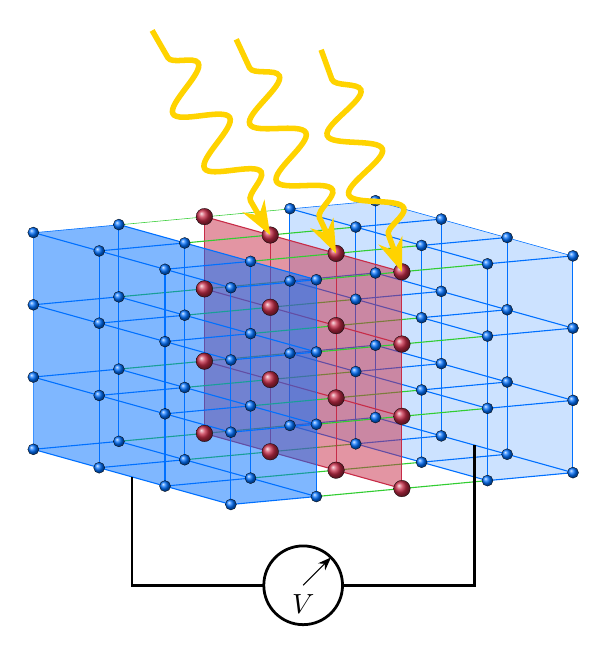
\begin{tikzpicture}[>=Stealth]
\begin{axis}[
axis lines=none,
view={150}{10},
xmin=0,xmax=4,
ymin=0,ymax=3,
zmin=-2,zmax=3,
xlabel=$x$,
ylabel=$y$,
zlabel=$z$,
scale=1
]

% right lead
% balls
\foreach \x in {0,1}
  \foreach \y in {0,1,...,3}
    \foreach \z in {0,1,...,3}
       \addplot3 [only marks,mark=ball,mark size=2pt,ball color=hblue,line width=0.1pt] coordinates{(\x,\y,\z)};
% lines
\pgfplotsinvokeforeach{0,1,...,3} {
   \draw[color=hblue] (axis cs:0,#1,0) -- (axis cs:0,#1,3);
   \draw[color=hblue] (axis cs:0,#1,0) -- (axis cs:1,#1,0);
   \draw[color=hblue] (axis cs:0,#1,1) -- (axis cs:1,#1,1);
   \draw[color=hblue] (axis cs:0,#1,2) -- (axis cs:1,#1,2);
   \draw[color=hblue] (axis cs:0,#1,3) -- (axis cs:1,#1,3);
};
\pgfplotsinvokeforeach{0,1,...,3} {
   \draw[color=hblue] (axis cs:0,0,#1) -- (axis cs:0,3,#1);
};
\pgfplotsinvokeforeach{0,1,...,3} {
   \draw[color=hblue] (axis cs:1,#1,0) -- (axis cs:1,#1,3);
};
\pgfplotsinvokeforeach{0,1,...,3} {
   \draw[color=hblue] (axis cs:1,0,#1) -- (axis cs:1,3,#1);
};
% bottom
% \fill[color=hblue,opacity=0.2] (axis cs:1,0,0) -- (axis cs:0,0,0) -- (axis cs:0,3,0) -- (axis cs:1,3,0) -- cycle;
% back
% \fill[color=hblue,opacity=0.2] (axis cs:1,0,0) -- (axis cs:0,0,0) -- (axis cs:0,0,3) -- (axis cs:1,0,3) -- cycle;
% front
\fill[color=hblue,opacity=0.2] (axis cs:1,0,0) -- (axis cs:1,3,0) -- (axis cs:1,3,3) -- (axis cs:1,0,3) -- cycle;
% left side
\fill[color=hblue,opacity=0.2] (axis cs:1,3,0) -- (axis cs:0,3,0) -- (axis cs:0,3,3) -- (axis cs:1,3,3) -- cycle;
% top
\fill[color=hblue,opacity=0.2] (axis cs:1,3,3) -- (axis cs:0,3,3) -- (axis cs:0,0,3) -- (axis cs:1,0,3) -- cycle;

   
% interface right-center
\pgfplotsinvokeforeach{0,1,...,3} {
   \draw[color=hgreen] (axis cs:1,#1,0) -- (axis cs:2,#1,0);
   \draw[color=hgreen] (axis cs:1,#1,1) -- (axis cs:2,#1,1);
   \draw[color=hgreen] (axis cs:1,#1,2) -- (axis cs:2,#1,2);
   \draw[color=hgreen] (axis cs:1,#1,3) -- (axis cs:2,#1,3);
};


% central layer
\fill[color=hred,opacity=0.5] (axis cs:2,0,0) -- (axis cs:2,3,0) -- (axis cs:2,3,3) -- (axis cs:2,0,3) -- cycle;
% lines
\pgfplotsinvokeforeach{0,1,...,3} {
   \draw[color=hred] (axis cs:2,#1,0) -- (axis cs:2,#1,3);
};
\pgfplotsinvokeforeach{0,1,...,3} {
   \draw[color=hred] (axis cs:2,0,#1) -- (axis cs:2,3,#1);
};
% balls
\foreach \y in {0,1,...,3}
  \foreach \z in {0,1,...,3}
     \addplot3 [only marks,mark=ball,mark size=3pt,ball color=hred,line width=0.1pt] coordinates{(2,\y,\z)};


% interface center-left
\pgfplotsinvokeforeach{0,1,...,3} {
   \draw[color=hgreen] (axis cs:2,#1,0) -- (axis cs:3,#1,0);
   \draw[color=hgreen] (axis cs:2,#1,1) -- (axis cs:3,#1,1);
   \draw[color=hgreen] (axis cs:2,#1,2) -- (axis cs:3,#1,2);
   \draw[color=hgreen] (axis cs:2,#1,3) -- (axis cs:3,#1,3);
};


% left lead
% balls
\foreach \x in {3,4}
  \foreach \y in {0,1,...,3}
    \foreach \z in {0,1,...,3}
       \addplot3 [only marks,mark=ball,mark size=2pt,ball color=hblue,line width=0.1pt] coordinates{(\x,\y,\z)};
% lines
\pgfplotsinvokeforeach{0,1,...,3} {
   \draw[color=hblue] (axis cs:3,#1,0) -- (axis cs:3,#1,3);
   \draw[color=hblue] (axis cs:3,#1,0) -- (axis cs:4,#1,0);
   \draw[color=hblue] (axis cs:3,#1,1) -- (axis cs:4,#1,1);
   \draw[color=hblue] (axis cs:3,#1,2) -- (axis cs:4,#1,2);
   \draw[color=hblue] (axis cs:3,#1,3) -- (axis cs:4,#1,3);
};
\pgfplotsinvokeforeach{0,1,...,3} {
   \draw[color=hblue] (axis cs:3,0,#1) -- (axis cs:3,3,#1);
};
\pgfplotsinvokeforeach{0,1,...,3} {
   \draw[color=hblue] (axis cs:4,#1,0) -- (axis cs:4,#1,3);
};
\pgfplotsinvokeforeach{0,1,...,3} {
   \draw[color=hblue] (axis cs:4,0,#1) -- (axis cs:4,3,#1);
};
% bottom
% \fill[color=hblue,opacity=0.5] (axis cs:4,0,0) -- (axis cs:3,0,0) -- (axis cs:3,3,0) -- (axis cs:4,3,0) -- cycle;
% back
% \fill[color=hblue,opacity=0.5] (axis cs:4,0,0) -- (axis cs:3,0,0) -- (axis cs:3,0,3) -- (axis cs:4,0,3) -- cycle;
% front
\fill[color=hblue,opacity=0.5] (axis cs:4,0,0) -- (axis cs:4,3,0) -- (axis cs:4,3,3) -- (axis cs:4,0,3) -- cycle;
% left side
\fill[color=hblue,opacity=0.5] (axis cs:4,3,0) -- (axis cs:3,3,0) -- (axis cs:3,3,3) -- (axis cs:4,3,3) -- cycle;
% top
\fill[color=hblue,opacity=0.5] (axis cs:4,3,3) -- (axis cs:3,3,3) -- (axis cs:3,0,3) -- (axis cs:4,0,3) -- cycle;


% coordinates for light
\coordinate (top1) at (axis cs:2,1,3);
\coordinate (top2) at (axis cs:2,2,3);
\coordinate (top3) at (axis cs:2,3,3);


% volt-meter lines
\coordinate (leftlead) at (axis cs:4,1.5,0);
\coordinate (belowleftlead) at (axis cs:4,1.5,-1.5);
\coordinate (rightlead) at (axis cs:0,1.5,0);
 
\draw[line width=1pt] let 
      \p1=(leftlead),
      \p2=(belowleftlead),
      \p3=(rightlead)
in
      (leftlead) -- (belowleftlead) -- (\x3,\y2) -- (rightlead);

\end{axis}

% volt-meter display
\filldraw[draw=black,fill=white,line width=1pt] let 
      \p1=(belowleftlead),
      \p2=(rightlead)
in
      ($ (\x1/2.,\y1)+(\x2/2.,0) $) circle (0.5);
\draw[->] let 
      \p1=(belowleftlead),
      \p2=(rightlead)
in
      ($ (\x1/2.,\y1)+(\x2/2.,0) $) -- node[at start,below] {$V$} ($ (\x1/2.,\y1)+(\x2/2.,0)+(0.35355,0.35355) $);

% cw-light
\draw [->,>=Stealth,line width=2pt,decorate,decoration={snake,amplitude=0.3cm,segment length=0.8cm,pre length=0.4cm,post length=0.4cm},draw=hyellow] ($ (top1)+(120:3) $) -- (top1);
\draw [->,>=Stealth,line width=2pt,decorate,decoration={snake,amplitude=0.3cm,segment length=0.8cm,pre length=0.4cm,post length=0.4cm},draw=hyellow] ($ (top2)+(115:3) $) -- (top2);
\draw [->,>=Stealth,line width=2pt,decorate,decoration={snake,amplitude=0.3cm,segment length=0.8cm,pre length=0.4cm,post length=0.4cm},draw=hyellow] ($ (top3)+(110:3) $) -- (top3);

% pulsed light
% \begin{scope}[decoration={markings,
% mark=at position 0.0 with {{\arrowreversed[hyellow,xshift=-6]{Stealth}}}},
% domain=-1.6:1.5,samples=300,xshift=8.4cm,yshift=4.6cm,rotate=110]
% \draw[postaction={decorate},draw=hyellow,line width=2pt] plot (\x,{0.8*exp(-\x*\x/(2.*0.3))*sin(10.*\x r)});
% \end{scope}

\end{tikzpicture}
\end{document}
